\begin{figure}[!htb]
	\centering
	\begin{subfigure}{0.45\textwidth}
		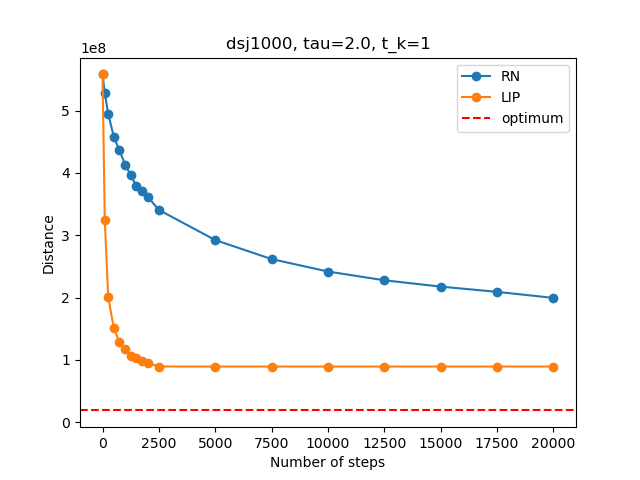
\includegraphics[width=\textwidth]{img/dsj1000_temp=2.0_cool=1.0}
		\subcaption{dsj1000, $t_k=1$.}
	\end{subfigure}
	\begin{subfigure}{0.45\textwidth}
		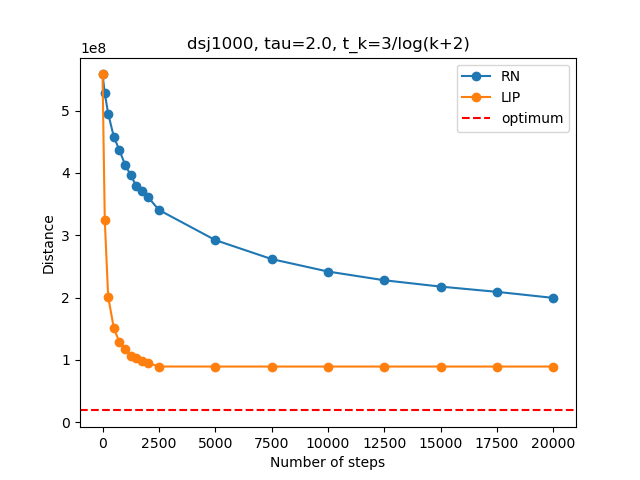
\includegraphics[width=\textwidth]{img/dsj1000_temp=2.0_cool=2.73}
		\subcaption{dsj1000, $t_k=\frac{3}{\log(k+2)}$.}
	\end{subfigure}
	\caption{Comparing RN and LIP for \textit{dsj1000} with different cooling parameters.}
\end{figure}